\chapter{Approximations}
\section{The Variational Principle}
\subsection{Theorem}
Suppose you want to find the ground state energy $E_g$ for a system described by the Hamiltonian $H$, but you are unable to solve the time-dependent Schrodinger equation. Pick any normalised function $\psi$ whatsoever, then,
\begin{equation}
	E_g\le\langle\psi|H|\psi\rangle\equiv\langle H\rangle
\end{equation}
The expectation value of $H$ in the tate $\psi$ is certain to overestimate the ground-state energy. If $\psi$ is an excited state, then it is obvious that the energy is greater than the ground state energy, but the theorem states that the same holds for any $\psi$ whatsoever.

\subsection{Proof}
Since the eigenfunctions of $H$ form a complete set, we can express $\psi$ as a linear combination of them,
\begin{equation*}
	\psi=\sum_{n}^{}c_n\psi_n, \; \text{with} \, H\psi_n=E_n\psi_n
\end{equation*}

Since $\psi$ is normalized,
\begin{equation*}
	1=\braket{\psi}{\psi}=\langle \sum_{m}^{}c_m\psi_m|\sum_{n}^{}c_n\psi_n\rangle=\sum_{m}^{}\sum_{n}^{}c^*_mc_n\langle\psi_m|\psi_n\rangle=\sum_{n}^{}|c_n|^2
\end{equation*}
This is under the assumption that the eigenfuctions have been orthornormalized. Meanwhile,
\begin{equation*}
	\langle H\rangle=\langle \sum_{m}^{}c_m\psi_m|H\sum_{n}^{}c_n\psi_n\rangle=\sum_{m}^{}\sum_{n}^{}c^*_mE_nc_n\langle\psi_m|\psi_n\rangle=\sum_{n}^{}E_n|c_n|^2
\end{equation*}
By defintion, ground state energy is the smallest eigenvalue, so $E_g\le E_n$, and hence,
\begin{equation*}
	\langle H\rangle\ge E_g\sum_{n}^{}|c_n|^2=E_g
\end{equation*}

\subsection{The Ground State of Helium}
The helium atom consists of two electrons in orbit around a nucleus containing two protons, and neutrons, but these are irrelevant as we are only considering charge here. The Hamiltonian for this system, ignoring fine structure and smaller corrections is,
\begin{equation}
	H=-\frac{\hbar^2}{2m}(\nabla^2_1+\nabla^2_2)-\frac{e^2}{4\pi\epsilon_0}\left(\frac{2}{r_1}+\frac{2}{r_2}-\frac{1}{|\textbf{r}_1-\textbf{r}_2|}\right)
\end{equation}

The ground state energy has been experimentally found out to be,
\begin{equation*}
	E_g=-78.975eV
\end{equation*}
We are trying to reproduce this value theoretically. This problem as no exact solution due to the electron-electron repulsion,
\begin{equation}
	V_{ee}=\frac{e^2}{4\pi\epsilon_0}\frac{1}{|\textbf{r}_1-\textbf{r}_2|}
\end{equation}
Ignoring this term, $H$ splits into two independent hydrogen Hamiltonians, and the exact solution is just the product of hydrogenic wave functions,
\begin{equation}
	\psi_0(\textbf{r}_1,\textbf{r}_2)\equiv\psi_{100}(\textbf{r}_1)\psi_{100}(\textbf{r}_2)=\frac{8}{\pi a^3}e^{-2(r_1+r_)/a}
\end{equation}
and the energy is $8E_!=-109 eV$. We can see that this isnt accurate.\\
To get a better approximation for $E_g$, we will apply the variational principle using $\psi_0$ as the trial wave function.
\begin{equation}
	H\psi_0=(8E_1+V_{ee})\psi_0
\end{equation}
Thus,
\begin{equation}
	\langle H\rangle=8e_1+\langle V_{ee}\rangle
\end{equation}
Where,
\begin{equation}
	\langle V_{ee}\rangle=\left(\frac{e^2}{4\pi\epsilon_0}\right)\left(\frac{8}{\pi a^3} \right)^2\int_{}^{}\frac{e^{-2(r_1+r_)/a}}{|\textbf{r}_1-\textbf{r}_2|}d^3\textbf{r}_1d^3\bm{r}_2
\end{equation}
\newpage
The choice of coordinates is as given below,
\begin{center}
	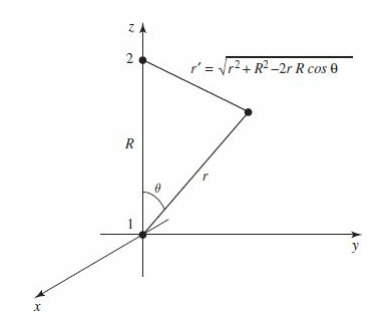
\includegraphics[scale=0.5]{coordinate}
\end{center}
Integral $\bm{r}_2$ is done first. From law of cosines,
\begin{equation}
	|\textbf{r}_1-\textbf{r}_2|=\sqrt{r_1^2+r_2^2-2r_1r_2cos\theta_2}
\end{equation}
And hence,
\begin{equation}
	I_2\equiv\frac{e^{-4r_2/a}}{|\textbf{r}_1-\textbf{r}_2|}=\int\frac{e^{-4r_2/a}}{\sqrt{r_1^2+r_2^2-2r_1r_2cos\theta_2}}r_2^2sin\theta_2dr_2\theta_2d\phi_2
\end{equation}
The $\phi_2$ integral equates to $2\pi$, the $\theta_2$ integral is,

\begin{equation*}
	\int_{0}^{\pi}\frac{sin\theta_2}{\sqrt{r_1^2+r_2^2-2r_1r_2cos\theta_2}}d\theta_2=\frac{\sqrt{r_1^2+r_2^2-2r_1r_2cos\theta_2}}{r_1r_2}\Big\rvert^\pi_0
\end{equation*}

\begin{equation}
	=\frac{1}{r_1r_2}[(r_1+r_2)-(r_1-r_2)]= 
	\begin{cases}
		2/r_1, & \text{if}\ r_2<r_1 \\
		2/r_2, & \text{if}\ r_2>r_1
	\end{cases}
\end{equation}

Thus,
\begin{equation*}
	I_2=4\pi\left(\frac{1}{r_1}\int_{0}^{r_1}e_{-4r_2/a}r_2^2dr_2+\int_{r_1}^{\infty}e^{-4r_2/a}r_2dr_2\right)
\end{equation*}
\begin{equation}
	=\frac{\pi a^3}{8r_1}\left[1-\left(1+\frac{2r_1}{a}e^{-4r_1/a}\right)\right]
\end{equation}

It then follows that $\langle V_{ee}\rangle$ is equal to,
\begin{equation*}
	\left(\frac{e^2}{4\pi\epsilon_0}\right)\left(\frac{8}{\pi a^3} \right)\int \frac{\pi a^3}{8r_1}\left[1-\left(1+\frac{2r_1}{a}e^{-4r_1/a}\right)\right]e^{-4r_1/a}r_1sin\theta_1 dr_1 d\theta_1 d\phi_1
\end{equation*}

The angular integrals are easy ($4\pi$) and the $r_1$ integral becomes,
\begin{equation*}
	\int_{0}^{\infty}\left[re^{-4r/a}-\left(r+\frac{2r^2}{a}\right)e^{-8r/a}\right]dr=\frac{5a^2}{128}
\end{equation*}

Finally,
\begin{equation}
	\langle V_{ee}\rangle=\frac{5}{4a}\left(\frac{e^2}{4\pi\epsilon_0}\right)=-\frac{5}{2}E_1=34 eV
\end{equation}
And therefore,
\begin{equation}
	\langle H \rangle=-109 eV+34eV=-75eV
\end{equation}

This is fairly accurate, but we can improve the result by thinking of a better trial wavefunction. Taking that on average, each electron represents a cloud of negative charge that partially shields the nucleus, so that the other electon sees an effective nucler charge that is somewhat less than 2.\\
This suggests that we use a trial function of the form,
\begin{equation}
	\psi_1(\bm{r}_1\bm{r}_2)\equiv\frac{Z^3}{\pi a^3}e^{-Z(r_1+r_2)/a}
\end{equation}
We vary $Z$ as a variational parameter, picking the value that minimizes $\langle H\rangle$.\\
The wavefunction is an eigenstate of the unperturbed hamiltonian, but with $Z$, instead of 2 in the couloumb terms. We rewrite $H$,
\begin{multline}
	H=\frac{\hbar^2}{2m}(\nabla^2_1+\nabla^2_2)-\frac{e^2}{4\pi\epsilon_0}\left(\frac{Z}{r_1}+\frac{Z}{r_2}\right)\\
	+\frac{e^2}{4\pi\epsilon_0}\left(\frac{(Z-2)}{r_1}+\frac{(Z-2)}{r_2}+\frac{1}{|\bm{r}_1-\bm{r_2}|}\right)
\end{multline}

The expectation value of $H$ is evidently,
\begin{equation}
	\langle H\rangle=2Z^2E_1+2(Z-2)\left(\frac{e^2}{4\pi\epsilon_0}\right)\langle\frac{1}{r}\rangle+\left\langle V_{ee}\right\rangle
\end{equation}
Here the $\langle<1/r\rangle$ is the expectation value of $1/r$ n the hydrogenic ground state $\psi_{100}$, 
\begin{equation}
	\left\langle \frac{1}{r}\right\rangle=\frac{Z}{a}
\end{equation}

Now the expectation value of $V_{ee}$ is,
\begin{equation}
	\langle V_{ee}\rangle =\frac{5Z}{8a}\left(\frac{e^2}{4\pi\epsilon_0}\right)=-\frac{5Z}{4}E_1
\end{equation}

Putting everything together,
\begin{equation}
	\langle H \rangle=[2Z^2-4Z(Z-2)-(5/4)Z]E_1=[-2Z^2+(27/4)Z]E_1
\end{equation}
According to the variational principle, this quantity exceeds $E_g$ for any value of $Z$. The lowest upper bound occurs when $\langle H \rangle$ is minimised,
\begin{equation}
	\frac{d}{dZ}\langle H \rangle=[-4Z+(27/4)]E_1=0
\end{equation}
from which it follows that,
\begin{equation}
	Z=\frac{27}{16}=1.69
\end{equation}
This says that the other electron partially screens the nucleus, reducing its effective charge from 2 to 1.69. Substituting this in Z, we find,
\begin{equation}
	\langle H \rangle=\frac{1}{2}\left(\frac{3}{2}^6\right)E_1=-77.5eV
\end{equation}

Hence we see that the ground state of helium has been calculated with great precision. We can improve this by selecting better trial wavefunctions, but we do not require that since we have already reached within 2\% of the correct answer.
\subsection{The Hydrogen Molecule Ion}
Another classic application of the variational principle is to the hydrogen molecule ion, H , consisting of a
single electron in the Coulomb field of two protons . Assuming for the moment that the
protons are fixed in position, a specified distance R apart, although one of the most interesting byproducts of
the calculation is going to be the actual value of R. The Hamiltonian is,
\begin{equation}
	H=\frac{\hbar^2}{2m}\nabla^2-\frac{e^2}{4\pi\epsilon_0}\left(\frac{1}{r}+\frac{1}{r'}\right)
\end{equation}

Where $r$ and $r'$ are the distances to the electron from the respective protons. Next we try to guess a reasonable trial wavefunction, by taking a hydrogen atom in its ground state,
\begin{equation}
	\psi_0(r)=\frac{1}{\sqrt{\pi a^3}}e^{-r/a}
\end{equation}

bringing the second proton in from “infinity,” and nailing it down a distance R away. If R is substantially
greater than the Bohr radius, the electron’s wave function probably isn’t changed very much. But we would
like to treat the two protons on an equal footing, so that the electron has the same probability of being
associated with either one. This suggests that we consider a trial function of the form,
\begin{equation}
	\psi=A[\psi_0(r)+\psi_0(r')]
\end{equation}
Normalising this wave function,
\begin{equation}
	1=\int|\psi|^2d^3r=|A|^2\left[\psi_0(r)^2d^3\bm{r}+\int\psi_0(r')^2+2\int\psi_0(r)\psi_0(r')d^3r\right]
\end{equation}
Evaluating the integrals give the normalisation factor to be,
\begin{equation}
	|A|^2=\frac{1}{2(1+I)}
\end{equation}
Where $I$ is,
\begin{equation}
	I=e^{-R/a}\left[1+\frac{R}{a}+\frac{1}{3}\left(\frac{R}{a}\right)^2\right]
\end{equation}

Now computing the expectation value of the Hamiltonian in the trial state $\psi$,
\begin{equation}
	\langle H\rangle=\left[1+2\frac{(D+X)}{1+I}\right]E_1
\end{equation}
According to the variational principle,
\begin{equation}
	V_{pp}=\frac{e^2}{4\pi\epsilon_0}\frac{1}{R}=-\frac{2a}{R}E_1
\end{equation}
Thus the total energy of the system, in the units of $-E_1$, and expressed as a function of $x\equiv R/\alpha$, is less than,
\begin{equation}
	F(x)=-1+\frac{2}{x}\left\{\frac{(1-(2/3)x^2)e^{-x}+(1+x)e^{-2x}}{1+(1+x+(1/3)x^2)e^{-x}}\right\}
\end{equation}

Plotting this function,
\begin{center}
	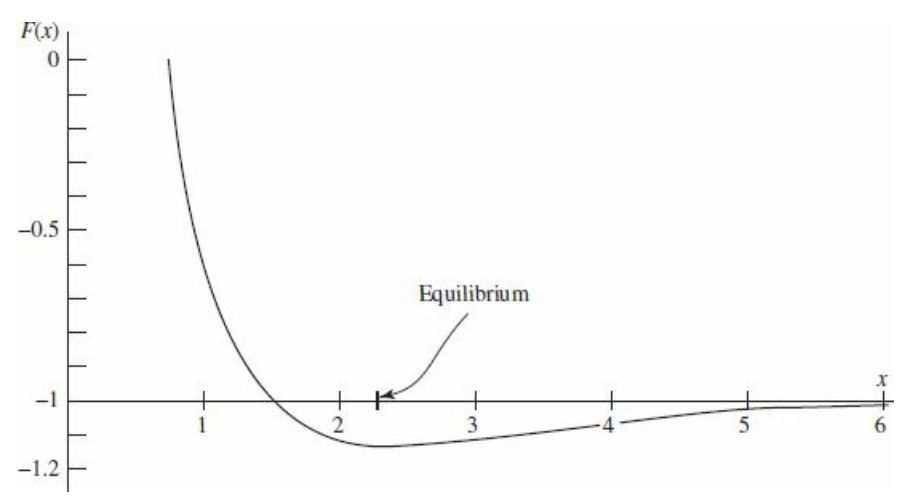
\includegraphics[scale=0.4]{variational}
\end{center}

Evidently bonding does occur, for there exists a region in which the graph goes below -1 , indicating that the energy is less than that of a neutral atom plus a free proton.

\newpage


\section{The WKB Approximation}
\subsection{Introduction}
The WKB (Wentzel, Kramers, Brillouin)1 method is a technique for obtaining approximate solutions to the
time-independent Schrödinger equation in one dimension (the same basic idea can be applied to many other
differential equations, and to the radial part of the Schrödinger equation in three dimensions). It is particularly
useful in calculating bound state energies and tunneling rates through potential barriers.
Imagine a particle of energy E moving through a region where the potential $V(x)$ is a constant. if $E>V$, the wavefunction is of the form,
\begin{equation*}
	\psi(x)=Ae^{\pm ikx}, \; \text{with}\; k\equiv\sqrt{2m(E-V)/\hbar}
\end{equation*}

The plus sign indicates that the particle is traveling to the right, and the minus sign means it is going to the
left (the general solution, of course, is a linear combination of the two). The wave function is oscillatory, with
fixed wavelength and unchanging amplitude . Now suppose that the potential is not constant, but
varies rather slowly in comparison to $\lambda$ , so that over a region containing many full wavelengths the potential is
essentially constant. Then it is reasonable to suppose that $\psi$ remains practically sinusoidal, except that the wavelength and the amplitude change slowly with x. This is the inspiration behind the WKB approximation.
In effect, it identifies two different levels of x-dependence: rapid oscillations, modulated by gradual variation in amplitude and wavelength.\\
If $E<V$,
\begin{equation*}
	\psi(x)=Ae^{\pm kx}, \; \text{with}\; k\equiv\sqrt{2m(V-E)/\hbar}
\end{equation*}

If $V(x)$ is not constant, but varies slowly in comparison with $1/k$, the solution remains practically exponential. The approximation fails at the classical turning point, where $E\approx V$, where $\lambda$ goes to infinity.

\subsection{The Classical Region}
The Schrodinger equation,
\begin{equation*}
	-\frac{\hbar^2}{2m}\frac{d^2\psi}{dx^2}+V(x)\psi=E\psi
\end{equation*}

can be rewritten as,
\begin{equation}
	\frac{d^2\psi}{dx^2}=-\frac{p^2}{\hbar^2}\psi
\end{equation}
where,
\begin{equation}
	p(x)\equiv\sqrt{2m[E-V(x)]}
\end{equation}
is the classical formula for momentum of a particle with total energy $E$ and potential energy $V(x)$. We assume that $E>V$, and this is the classical region and the particle is confined to this range of x. Writing the complex function $\psi$ in terms of amplitude and phase,
\begin{equation}
	\psi(x)=A(x)e^{i\phi(x)}
\end{equation}

Using a prime to denote the derivative with respect to $x$, we find,
\begin{equation*}
	\frac{d\psi}{dx}=(A'+iA\phi')e^{i\phi}
\end{equation*}

And,
\begin{equation}
	\frac{d^2\psi}{dx^2}=[A''+2iA'\phi'+iA\phi''-A(\phi')^2]
\end{equation}
Putting this in equation (32)
\begin{equation}
	\frac{d^2\psi}{dx^2}=[A''+2iA'\phi'+iA\phi''-A(\phi')^2]= -\frac{p^2}{\hbar^2}A
\end{equation}

We can split this into two parts, the real and imaginary,
\begin{equation}
	A''-A(\phi')^2=\frac{-p^2}{\hbar^2}A, \; \text{or} \; A''=A\left[(\phi')^2-\frac{p^2}{\hbar^2}\right]
\end{equation}
And,
\begin{equation}
	2A'\phi'+ A\phi''=0, \; \text{or} \; (A^2\phi')'=0
\end{equation}

From this we get that,
\begin{equation}
	\phi(x)=\pm\frac{1}{\hbar}\int p(x)dx
\end{equation}
And then,
\begin{equation}
	\psi(x)\approxeq\frac{C}{\sqrt{p(x)}}e^{\pm \frac{1}{\hbar}\int p(x)dx}
\end{equation}
And that the general approximate solution will be a linear combination of two of these terms, one with each sign. See that,
\begin{equation}
	|\psi(x)|^2\approxeq\frac{|C|^2}{p(x)}
\end{equation}
Which says that the probability of finding a particle at point x is inversely proportional to the classical momentum at that point. Sometimes, the WKB approximation is derived from this semiclassical observation.

\subsection{Tunneling}
Now assuming that $E<V$, $p(x)$ becomes imaginary,
\begin{equation}
	\psi(x)\approxeq\frac{C}{\sqrt{|p(x)|}}e^{\pm \frac{1}{\hbar}\int |p(x)|dx}
\end{equation}
Take a problem of scattering from a rectangular barrier with a bumpy top, to the left of the barrier,
\begin{equation}
	\psi(x)=Ae^{ikx}+Be^{-ikx}
\end{equation}
To the right of the barrier,
\begin{equation}
	\psi{x}=Fe^{ikx}
\end{equation}
Where F is the transmitted amplitude and the tunneling probability is,
\begin{equation}
	T=\frac{|F|^2}{|A|^2}
\end{equation}
Our WKB approximation gives us,
\begin{equation}
	\psi(x)\approxeq \frac{C}{\sqrt{|p(x)|}}e^{\pm \frac{1}{\hbar}\int_{0}^{x} |p(x')|dx'} +\frac{D}{\sqrt{|p(x)|}}e^{\pm -\frac{1}{\hbar}\int_{0}^{x} |p(x')|dx'}
\end{equation}

If the barrier is sufficiently wide, the exponentially increasing term diminishes, and the relative amplitudes look like,
\begin{equation*}
	\frac{|F|}{|A|}\approx e^{\pm -\frac{1}{\hbar}\int_{0}^{\alpha} |p(x')|dx'}
\end{equation*}

So that,
\begin{gather}
	T\approxeq e^{-2\gamma}\\
	\gamma\equiv \frac{1}{\hbar}\int_{0}^{\alpha} |p(x')|dx'
\end{gather}


\subsection{The connection formulas}
We have obtained the wavefunctions for before and after the walls of the potential well, now to determine the region within the potential well, or at a turning point ($E=V$), shifting the axes so that the right hand turning point occurs at $x=0$, in the WKB approximation we have,
\begin{equation}
	\psi(x)\approxeq
	\begin{cases}
		\frac{1}{\sqrt{|p(x)|}}\left[Be^{ \frac{1}{\hbar}\int_{x}^{0} |p(x')|dx'} +Ce^{\pm -\frac{1}{\hbar}\int_{x}^{0} |p(x')|dx'}\right], \; \text{if}\; x<0 \\
		
		\frac{1}{\sqrt{|p(x)|}}De^{-\frac{1}{\hbar}\int_{0}^{x}|p(x')|dx'} \; \text{if} \; x>0
	\end{cases}
\end{equation}
We essentially patch the two WKB solutions, by using the connection formulas,
\begin{equation}
	B=-ie^{i\pi/4}D, \; \text{and}\; C=ie^{-i\pi/4}D
\end{equation}

Now providing the final wavefunction,
\begin{equation}
	\psi(x)\approxeq
	\begin{cases}
		\frac{-2D}{\sqrt{|p(x)|}}sin\left[ \frac{1}{\hbar}\int_{x}^{x^2} |p(x')|dx'+\frac{\pi}{4}\right],\; \text{if}\; x<x_2\\
		
		\frac{D}{\sqrt{|p(x)|}}e^{-\frac{1}{\hbar}\int_{x_2}^{x}|p(x')|dx'} \; \text{if} \; x>x_2
	\end{cases}
\end{equation}
Where $x_2$ is an arbitrary point.

\section{The Adiabatic Approximation}
\subsection{Adiabatic processes}
A gradual change in the external conditions characterises an adiabatic process. There are two characteristic times involved, $T_i$, the internal time, which governs the motion of the system itself and $T_e$, the external time regarding the change in external parameters.\\

Suppose that the Hamiltonian changes gradually from some initial form $H^i$ to some final form $H^f$, the adiabatic theorem states that if the particle was initially in the nth eigenstate of $H^i$, it will be carried under the Schrodinger equation into the nth eigenstate of $H^f$.\\

Take the example of a particle prepared in the ground state of an infinite square well,
\begin{equation}
	\psi^i(x)=\sqrt{\frac{2}{a}}\sin\left(\frac{\pi}{a}x\right)
\end{equation}

If we now gradually move the right wall out to 2a. the adiabatic theorem says that the particle will end up in the ground state of the expanded well,
\begin{equation}
	\psi^f(x)=\sqrt{\frac{1}{a}}\sin\left(\frac{\pi}{2a}x\right)
\end{equation}

Note that this change in Hamiltonian isnt small, like perturbation theory, the change can be as huge as needed, but the change should happen slowly is what the adiabatic approximation requires.

\subsection{Berry's Phase}
Now we discuss how the Adiabatic approximation is used in nonholonomic processes, where a system does not return to its original state when transported around a closed loop.\\
If the Hamiton is independent of time, then a particle which starts out in the $n$th eigenstate $\psi_n(x)$,
\begin{equation}
	H\psi_n(x)=E_n\psi_n(x)
\end{equation}
remains in the $n^{th}$ eignstate, simply picking up a phase factor,
\begin{equation}
	\Psi_n(x,t)=\psi_n(x)e^{-iE_nt/\hbar}
\end{equation}
But the adiabatic theorem states that when H changes gradually, the particle remains in the $n^th$ eignstate, even as the eigenfunction itself evolves,
\begin{equation}
	\Psi_n(x,t)=\psi_n(x,t)e^{-\frac{1}{\hbar}\int_{0}^{t}E_n(t')dt'}e^{i\gamma_n(t)}
\end{equation}
Where the term,
\begin{equation}
	\theta_n(t)\equiv-\frac{1}{\hbar}\int_{0}^{t}E_n(t')dt'
\end{equation}
Is the dynamic phase and the extra phase, $\gamma_n(t)$ is the geometric phase, which has its significance in the adiabatic theorem.\\
The net geometric phase change is usually given by,
\begin{equation}
	\gamma_n(t)=i\oint \langle\psi_n|\nabla_R\psi_n\rangle \cdot dR
\end{equation}

This is a line integral around a losed loop in parameter space, and its not zero. This is called Berry's phase, and it depends only on the path taken, not on how fast the path is traversed, meanwhile the dynamic phase depends critically on elapsed time